%%%%%%%%%%%%%%%%%%%%%%%%%%%%%%%%%%%%%%%%%%%%%%%%%%%%%%%%%%%%%%%%%%%%%%%%
%%%  THIS TEX FILE IS TO GENERATE PDF FILE FOR 
%%% 
%%%  COPYRIGHT (C) JIMMY LIN, 2013, UT AUSTIN
%%%%%%%%%%%%%%%%%%%%%%%%%%%%%%%%%%%%%%%%%%%%%%%%%%%%%%%%%%%%%%%%%%%%%%%%
\documentclass[11pt,a4paper]{article}
%%%%%%%%%%%%%%%%%%%%%%%%%%%%%%%%%%%%%%%%%%%%%%%%%%%%%%%%%%%%%%%%%%%%%%%%
%%%  PACKAGES USED IN THIS TEX SOURCE FILE
%%%%%%%%%%%%%%%%%%%%%%%%%%%%%%%%%%%%%%%%%%%%%%%%%%%%%%%%%%%%%%%%%%%%%%%%
\usepackage{geometry,amsthm,amsmath,graphicx,amssymb,fancyheadings}
\usepackage{epstopdf}
\usepackage[caption=false]{subfig}
\usepackage[]{mcode}
\usepackage[colorlinks,
            linkcolor=blue,
            anchorcolor=red,
            citecolor=green
            ]{hyperref}
% for my mac
\IfFileExists{/Users/JimmyLin/.latex/UTA_CS/JS.sty}{ 
    \usepackage{/Users/JimmyLin/.latex/UTA_CS/JS}
    \usepackage{/Users/JimmyLin/.latex/UTA_CS/JSASGN}
}{} 
% for UT's linux machine
\IfFileExists{/u/jimmylin/workspace/Configs/latex/UTA_CS/JS.sty}{
    \usepackage{/u/jimmylin/.latex/UTA_CS/JS} 
    \usepackage{/u/jimmylin/.latex/UTA_CS/JSASGN}
}{} 
%%%%%%%%%%%%%%%%%%%%%%%%%%%%%%%%%%%%%%%%%%%%%%%%%%%%%%%%%%%%%%%%%%%%%%%%
%%% MACROS CONTAINING THE FILE INFORMATION
%%%%%%%%%%%%%%%%%%%%%%%%%%%%%%%%%%%%%%%%%%%%%%%%%%%%%%%%%%%%%%%%%%%%%%%%
\renewcommand{\COURSE}{EE381V Large Scale Optimization}
\renewcommand{\LECTURER}{Sujay Sanghavi}
\renewcommand{\SECTION}{17350}
\renewcommand{\TASK}{Problem Set 4}
\renewcommand{\RELEASEDATE}{October 18, 2014}
\renewcommand{\DUEDATE}{October 23, 2014}
\renewcommand{\TIMECONSUME}{10 hours}
%%%%%%%%%%%%%%%%%%%%%%%%%%%%%%%%%%%%%%%%%%%%%%%%%%%%%%%%%%%%%%%%%%%%%%%%
%%% DOCUMENTATION STARTS FROM HERE 
%%%%%%%%%%%%%%%%%%%%%%%%%%%%%%%%%%%%%%%%%%%%%%%%%%%%%%%%%%%%%%%%%%%%%%%%
\begin{document}
%%%%%%%%%%%%%%%%%%%%%%%%%%%%%%%%%%%%%%%%%%%%%%%%%%%%%%%%%%%%%%%%%%%%%%%%
%% TITLE PAGE
%%%%%%%%%%%%%%%%%%%%%%%%%%%%%%%%%%%%%%%%%%%%%%%%%%%%%%%%%%%%%%%%%%%%%%%%
\begin{titlepage}
    \maketitle
\end{titlepage}
%%%%%%%%%%%%%%%%%%%%%%%%%%%%%%%%%%%%%%%%%%%%%%%%%%%%%%%%%%%%%%%%%%%%%%%%
%% CONTENT PAGE: TABLEOFCONTENTS, LISTOFTABLES, LIST OF FIGURES
%%%%%%%%%%%%%%%%%%%%%%%%%%%%%%%%%%%%%%%%%%%%%%%%%%%%%%%%%%%%%%%%%%%%%%%%
\renewcommand{\contentsname}{Table of Contents}
\begin{center} 
    \tableofcontents 
    %\listoftables 
    \listoffigures
\end{center}
\newpage
%%%%%%%%%%%%%%%%%%%%%%%%%%%%%%%%%%%%%%%%%%%%%%%%%%%%%%%%%%%%%%%%%%%%%%%%
%%% GENERAL DOCUMENTATION BEGINS 
%%%%%%%%%%%%%%%%%%%%%%%%%%%%%%%%%%%%%%%%%%%%%%%%%%%%%%%%%%%%%%%%%%%%%%%%

\part{Matlab and Computational Assignment}
\section{Conjugate Gradient Algorithm}
\subsection{$M_1$}
{\bf Command} to be executed in matlab:
\begin{verbatim}
    >> load ConjugateGradient.mat
    >> CGS(M1, b1, x)
\end{verbatim}
{\bf Plot}
\begin{figure}[h]
    \centering
    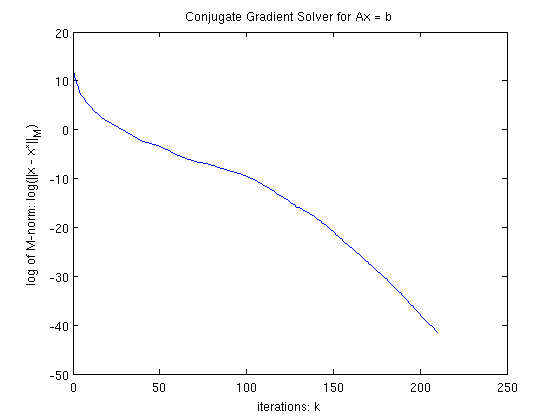
\includegraphics[width=4in,height=2.5in]{../ps4_matlab/M1.png}
    \caption{Conjugate Gradient Solver for $M_1$}
\end{figure}

\subsection{$M_2$}
{\bf Command} to be executed in matlab:
\begin{verbatim}
    >> load ConjugateGradient.mat
    >> CGS(M2, b2, x)
\end{verbatim}
{\bf Plot}
\begin{figure}[h]
    \centering
    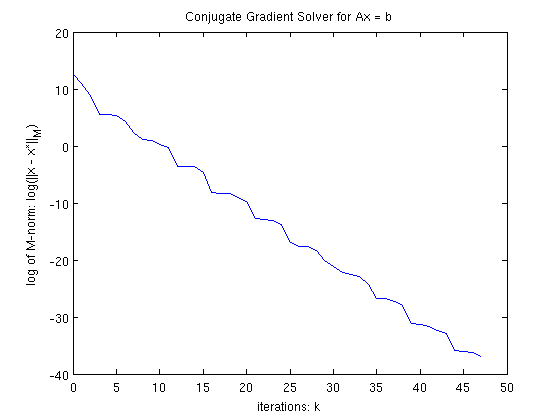
\includegraphics[width=4in,height=2.5in]{../ps4_matlab/M2.png}
    \caption{Conjugate Gradient Solver for $M_2$}
\end{figure}

\newpage
\section{Newton’s Method}
\subsection{plots for various $m$}
{\bf Command} to run:
\begin{verbatim}
    >> Newton(0, 'k-')
    >> hold on
    >> Newton(0.0001, 'k--')
    >> Newton(0.001, 'k:')
    >> Newton(0.1, 'k-.')
    >> Newton(0, 'k-')
\end{verbatim}

\noindent
{\bf Plots}
\begin{figure}[h]
    \centering
    \includegraphics[width=5in]{newton_method.eps}
\end{figure}
Note that the initial point here is $0.5 * ones(5, 1)$.

\subsection{Explanation}
From the figure, we can see that the $f_m(\cdot)$ goes to quadratic
convergence phrase with fewer number of iterations if $m$ is greater. The
intuitive explanation is that the larger $m$ will cause quadratic convergence
condition $|| \nabla f(x) || < \frac{m^2}{L}$ easier to satisfy. Note that one
extreme is when $m=0$, our newton method solver never goes into quadratic
convergence phrase (only linear convergence phrase).

\newpage
\section{Central Path}
\subsection{Find a function $F$}
\begin{align}
    F = -\sum_{i=1}^4 log(x_i) 
    - log (4 - x_1 - 3x_2 - x_4)
    - log (3 - 2x_1 - x_2)
    - log (3 - x_2 - 4x_3 - x_4)
\end{align}

\subsection{Find analytic center $x_F^*$}
\begin{align}
    x_F^* &= arg \min_{x\in dom F} F(x) \\
        &= (0.5488, 0.3091, 0.2543, 0.6485)
\end{align}

\subsection{Generate a central path}
The commands we used for generating a central path with various $\alpha$ 
\begin{verbatim}
    >> t_init = 5; alpha1=0.01; alpha2=0.1; alpha3=0.5; alpha4=1e-3;
    >> CP(t_init, alpha1, 'k-');
    >> hold on
    >> CP(t_init, alpha2, 'k--');
    >> CP(t_init, alpha3, 'k:');
    >> CP(t_init, alpha4, 'k-.');
\end{verbatim}

\subsection{Plot the error $log(|| x^{(k)} - x^*|| )$ w.r.t $k$}
In order to plot the errors, we first employ CVX to obtain the optimal feasible point $x^*$ by
\begin{verbatim}
    >> CVX_solve_CP
\end{verbatim}
For implementation details of this program, please go to appendix.

\noindent 
Then we have optimal feasible point for plotting $log(|| x^{(k)} - x^*|| )$
\begin{align}
    x^* = (0, 0, 0, 0)    
\end{align}

\noindent 
{\bf Plots}
\begin{figure}[h]
    \centering
    \includegraphics[width=4in]{CP_alphas.eps}
\end{figure}

\newpage
\section{Larger Linear Program}
\subsection{Find a function $F$}
For given $A^{m \times n}$
\begin{align}
    F = -\sum_{i=1}^N log(x_i) - \sum_{i=1}^{m} log (b - a_i^T x)
\end{align}

\subsection{Find analytic center $x_F^*$}
Newton's method start from $x_0 = 0.01 * ones(100, 1)$.
We first employ CVX to compute a feasible point and then use newton\_solver to
figure out the analytic center. Since it has 50 elements, we are not going to
post it here.

\subsection{Generate a central path}
Using similar commands with ones in response to previous question.

\subsection{Plot the error $log(|| x^{(k)} - x^*|| )$ w.r.t $k$}
{\bf Plot}
\begin{figure}[h]
    \centering
    \includegraphics[width=4in]{./CP_large.eps}
\end{figure}

\newpage
\section{Gradient and Newton}
{\bf Command} to be executed:
\begin{verbatim}
    >> Rosenbrock
\end{verbatim}

\noindent
{\bf Plot}
\begin{figure}[h]
    \centering
    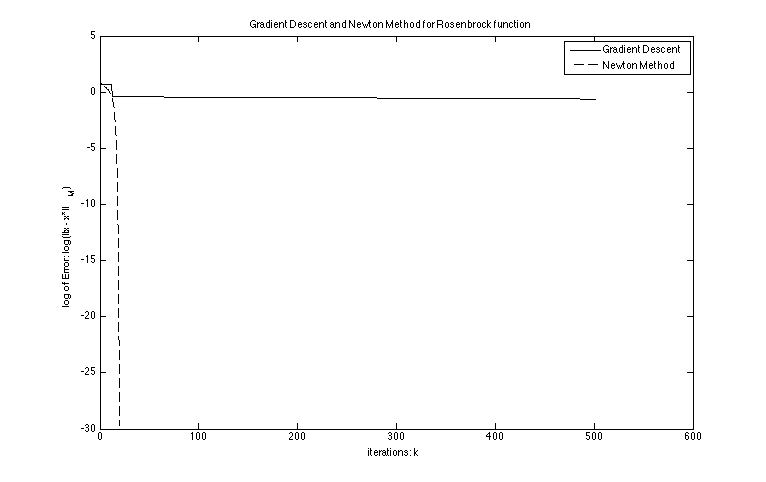
\includegraphics[width=5in]{Rosenbrock.eps}
    \caption{Gradient Descent and Newton Method on Rosenbrock function }
\end{figure}

\newpage
\part{Written Problems}
\section{$\alpha-$holder}
\newcommand{\dx}{\Delta x_{nt}}
Now we derive the rate of convergence with step size $t = 1$,
\begin{align}
    || \nabla f(x^+) ||_2 
    & = || \nabla f(x + \dx) - \nabla f(x) - \nabla^2 f(x) \dx ||_2 \\
    & = \bigg|\bigg| \int_0^1 \big( \nabla^2 f(x + t\dx) - \nabla^2 f(x) \big) \dx dt \bigg|\bigg|_2 \\
    & \leq  \int_0^1 || \big( \nabla^2 f(x + t\dx) - \nabla^2 f(x) \big) ||_2 \cdot ||\dx||_2 \cdot dt  \\
    & \leq  \int_0^1 H ||t\dx||_2^\alpha \cdot ||\dx||_2 \cdot dt  \\
    & = H || \dx ||_2^{1+\alpha} \cdot \frac{1}{1+\alpha} t^{1+\alpha} \Bigg|_0^1 \\
    & = \frac{H}{1+\alpha} || \dx ||_2^{1+\alpha} \\
    & = \frac{H}{1+\alpha} || \nabla^2 f(x)^{-1} \nabla f(x) ||_2^{1+\alpha} \\
    & \leq \frac{H}{(1+\alpha) m^{1+\alpha}} ||\nabla f(x) ||_2^{1+\alpha} \\
\end{align}
Thus, we can easily find a constant $C$, such that
\begin{align}
    C  \cdot || \nabla f(x^+) ||_2 \leq
    \bigg(C \cdot ||\nabla f(x) ||_2 \bigg) ^{1+\alpha}  \label{bound}
\end{align}
where $C = (\frac{H}{(1+\alpha) m^{1+\alpha}})^{-\alpha}$. \\
Recursively apply \eqref{bound} and simulate the same inference of (9.34) and
(9.35) in Boyd's book, we can conclude that once $|| \nabla f(x^{(k)}) || $ is
small enough, then the convergence will go into convergence phrase with order
at $1+\alpha$.

\newpage
\appendix
\section{Codes Printout}

\subsection{Conjugate Gradient Algorithm}
\lstinputlisting{../ps4_matlab/CGS.m}

\newpage
\subsection{Newton’s Method}
\lstinputlisting{../ps4_matlab/Newton.m}

\newpage
\subsection{Newton Solver For Central Path Generation}
\lstinputlisting{../ps4_matlab/Newton_solver.m}

\newpage
\subsection{Small Linear Program}
\lstinputlisting{../ps4_matlab/CP.m}

\newpage
\subsection{Larger Linear Program}
\lstinputlisting{../ps4_matlab/CP_large.m}

\newpage
\subsection{Gradient and Newton}
\lstinputlisting{../ps4_matlab/Rosenbrock.m}
%%%%%%%%%%%%%%%%%%%%%%%%%%%%%%%%%%%%%%%%%%%%%%%%%%%%%%%%%%%%%%%%%%%%%%%%
%%% General Documentation ends
%%%%%%%%%%%%%%%%%%%%%%%%%%%%%%%%%%%%%%%%%%%%%%%%%%%%%%%%%%%%%%%%%%%%%%%%
\end{document}
